\chapter{\textsc{Modélsation sous TINA}}
%%\section{\textsc{ Analyse du modèle à temps discret de l'ensemble (bloqueur d'ordre $0$, procédé en boucle ouverte) }}
%%\subsection{\textsc{La description sur les matrices d'état $ A_d,\hspace{1mm}B_d $ et $ C_d $ }}

\paragraph{} En premier lieu on commence par modéliser un RdP sous le logiciel TINA, puis on va extraire le fichier "Test\_MAL.ndr" dans le but d'éxécuter la moulinette en utilisant le terminal.\\\\
\textbf{Nota: } Le RdP modélisé ici est celui proposé par M ESTEBAN dans le but de le tester sur la maquette machine à laver à la toute fin.

	\begin{center}
	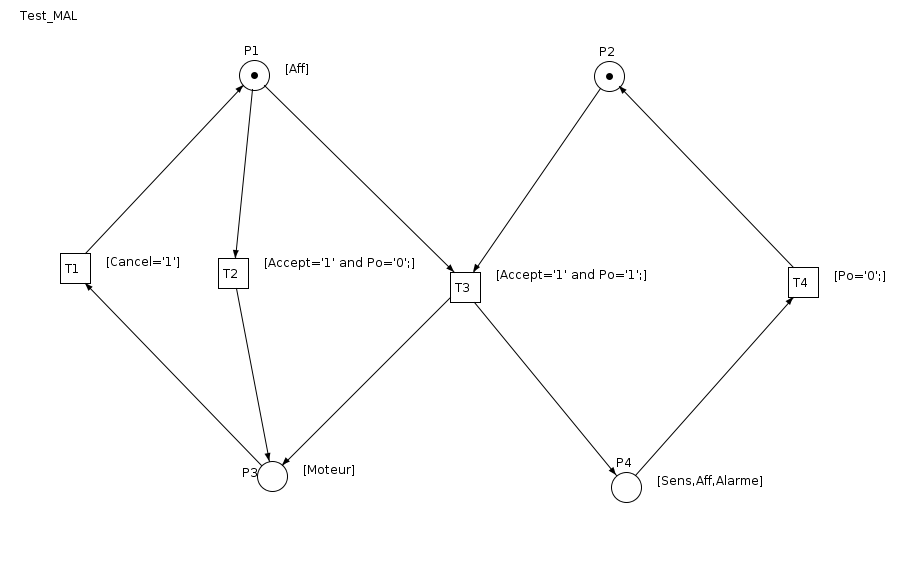
\includegraphics[scale=0.5]{Test_MAL.png}
	\captionof{figure}{\textit{RdP Test\_MAL proposé \\}}
	\label{fig1} 
	\end{center}	   

\chapter{\textsc{Mise en œuvre}}	
\section{\textsc{Développement de la fonction GenererBlocF.c}}

\paragraph{} Dans un premier temps, on crée les deux fichiers "package" et "entity" qu'on appelera $ package\_MAL.vhd $ et $entity\_place.vhd$ et enfin le fichier $evolution\_modele.vhd$\\[0.25 cm]

\begin{lstlisting}
#include "types.c"
#include <string.h>
#include<stdlib.h>

void GenererBlocF (Transition * PremiereTransition,Place * PremierePlace, char LeFichierEnVHDL[MAX_NOM]) {

	Transition * trans = PremiereTransition;
   	Place * pla = PremierePlace;
	FILE * f1; //fichier evolution_modele
	FILE * f2; // fichier du package
	FILE * f3; // fichier de l'entite
	
	f1=fopen(LeFichierEnVHDL,"w");
	f2=fopen("package_MAL.vhd","w");
	f3=fopen("entity_place.vhd","w");
\end{lstlisting}

\paragraph{} On remplit le fichier package:\\[0.25 cm]

\begin{lstlisting}
//Remplissage du fichier package	
fprintf(f2,"package MAL is \n \t component place_b \n \t \t port(ck, ra0_int, ra1_init, activer, desactiver : in std_logic ;\n \t \t \t marque : out std_logic) ;\n ");
fprintf(f2,"\tend component ; \n");
fprintf(f2,"end MAL ;\n\n");
fclose(f2);
\end{lstlisting}

\paragraph{} Le résultat est le suivant:\\[0.25 cm]

\begin{lstlisting}[style=vhdl]
package MAL is 
 	 component place_b 
 	 	 port(ck, ra0_int, ra1_init, activer, desactiver : in std_logic ;
 	 	 	 marque : out std_logic) ;
 	end component ; 
end MAL ;
\end{lstlisting}

\paragraph{} On remplit le fichier entity:\\[0.25 cm]

\begin{lstlisting}
//Remplissage du fichier ENTITY
fprintf(f3,"entity place_b is\nport (ck \t\t: in std_logic ;\n");
fprintf(f3,"\tra0_init, ra1_init \t: in std_logic ;\n");
fprintf(f3,"\tactiver, desactiver \t: in std_logic ;\n");
fprintf(f3,"\tmarque \t\t: out std_logic ;\n");
fprintf(f3,"end place_b;\n\n");
fprintf(f3,"architecture archi_place of place_b is\n");
fprintf(f3,"begin\n");
fprintf(f3,"\tprocess (ck, ra0_init, ra1_init, activer, desactiver)\n");
fprintf(f3,"\tbegin\n");
fprintf(f3,"\t\tif (ra0_init = '1') then marque <= '0';\n");
fprintf(f3,"\t\telsif (ra1_init = '1') then marque <= '1';\n");
fprintf(f3,"\t\telsif (ck'event and ck = '1') then \n");
fprintf(f3,"\t\t\tif (activer = '1') then marque <= '1';\n");
fprintf(f3,"\t\t\telsif (desactiver <= '1') then marque <= '0'; \n");
fprintf(f3,"\t\t\tend if ;\n");
fprintf(f3,"\t\tend if ;\n");
fprintf(f3,"\tend process ;\n");
fprintf(f3,"end archi_place ;\n\n");
fclose(f3);
\end{lstlisting}
\break
\paragraph{} Le résultat est le suivant:\\[0.25 cm]

\begin{lstlisting}[style=vhdl]
entity place_b is
port (ck 		: in std_logic ;
	ra0_init, ra1_init 	: in std_logic ;
	activer, desactiver 	: in std_logic ;
	marque 		: out std_logic ;
end place_b;

architecture archi_place of place_b is
begin
	process (ck, ra0_init, ra1_init, activer, desactiver)
	begin
		if (ra0_init = '1') then marque <= '0';
		elsif (ra1_init = '1') then marque <= '1';
		elsif (ck'event and ck = '1') then 
			if (activer = '1') then marque <= '1';
			elsif (desactiver <= '1') then marque <= '0'; 
			end if ;
		end if ;
	end process ;
end archi_place ;
\end{lstlisting}

\paragraph{} Enfin on remplit le fichier commenté evolution\_modele:
\begin{lstlisting}
	//Remplissage du fichier Bloc F
	fprintf(f1,"------bloc F-------\n");

	int i,j,nb,o,same;	
	char *Nom_p;
	Arc *arc_So;
	Arc *arc_En;
	Arc *arc_N;

	//parcours de le liste Place
	do{  
		same=0;
	
		//Remplissage de la partie activation des places 
        	Nom_p=pla->Nom;	
		fprintf(f1,"a_%s <= '1' when ",Nom_p);	

		//parcours de le liste Transition
 		do{
			nb=trans->NbPlacesSortie;//retenir le nombre de places que va activer la transition actuelle 
    			o=trans->NbPlacesEntree; //retenir le nombre de places qui peuvent affranchir la transition actuelle 
    			arc_So=trans->ArcsSortants; //retenir le nombre d'arcs sortant de la transition actuelle 
    			arc_En=trans->ArcsEntrants; //retenir le nombre d'arcs entrant des places vers la transition actuelle 
				
			// parcours du champs "ArcsSortants" de la transition actuelle
        	  	for(i=0;i<nb;i++){ 
				if(strcmp (arc_So->Place ,Nom_p) == 0 ){
			      		if(o==0){
						if(same!=0) fprintf(f1," or "); // On reste sur la meme ligne 
        	                              	fprintf(f1,"(");same=1;
        	                              	fprintf(f1,"%s)",trans->Predicat);
        	             		}
				        else{ 
						if(same!=0) fprintf(f1," or "); // On reste sur la meme ligne 
        	                        	fprintf(f1,"(");
						
						// parcours de la liste Arc
        	                        	for(j=0;j<o;j++) {
        	                          		fprintf(f1,"%s='1'",arc_En->Place);
				            		fprintf(f1," and ");
			                    		arc_En=arc_En->Suivant; 
        	                            		same=1;
        	                       	 	}
				        	fprintf(f1,"%s)",trans->Predicat);
        	              		} 			
			   	}
        	    		arc_So=arc_So->Suivant; 	     	
        	 	} 
 			trans=trans->Suivant;
 		} while(trans!=NULL);

 		trans = PremiereTransition;
		fprintf(f1," else '0';");
		fprintf(f1,"\n"); 

		//Remplissage de la partie desactivation des places 		
		same=0; 
		Nom_p=pla->Nom;	
		fprintf(f1,"d_%s <= '1' when",Nom_p);
		
		//parcours de le liste Transition
		do{ 
 			o=trans->NbPlacesEntree;
 			arc_En=trans->ArcsEntrants;
		
			// parcours du champs "ArcsEntrants" de la transition actuelle
 			for(i=0;i<o;i++){
				if (strcmp (arc_En->Place ,Nom_p) == 0){
        	        		if(nb==0){ 	
			        		fprintf(f1,"%s",trans->Predicat);
						same=1;
        	                	}
			        	else {
        	               			if(same!=0)fprintf(f1," or "); // On reste sur la meme ligne
        	                     		fprintf(f1," (");
        	     	             		arc_N=trans->ArcsEntrants;
			
						// parcours de la liste Arc
        	                     		for(i=0;i<o;i++){
				      			fprintf(f1,"%s='1' and ",arc_N->Place);
        	                      			arc_N=arc_N->Suivant;
							same=1;
        	                        }
				     	fprintf(f1," %s) ",trans->Predicat);                 
					}  
        	       		}
        	       arc_En=arc_En->Suivant;			  
        	       }                                    
		trans=trans->Suivant;
		} while(trans!=NULL); 
	
		trans = PremiereTransition;
		fprintf(f1,"else '0';");
		fprintf(f1,"\n\n");
		pla=pla->Suivant; 	
		} while( pla !=NULL);

		pla = PremierePlace;		
		fprintf(f1,"--marquage:\n\n");
		
		// Remplissage de la partie marquage en parcourant la liste Place
		do{
			Nom_p=pla->Nom;
			fprintf(f1,"place_%s: place_b port map (ck, r_%s, s_%s, a_%s, d_%s, %s);\n",Nom_p,Nom_p,Nom_p,Nom_p,Nom_p,Nom_p);
			pla=pla->Suivant;
		} while(pla !=NULL);
		fclose(f1);	
}
\end{lstlisting}
\break
\paragraph{} Le résultat est le suivant:\\[0.25 cm]

\begin{lstlisting}[style=vhdl]
------bloc F-------
a_p2 <= '1' when (p4='1' and Po='0') else '0';
d_p2 <= '1' when (p2='1' and p1='1' and  Accept='1' and Po='1') else '0';

a_p1 <= '1' when (p3='1' and Cancel='1') else '0';
d_p1 <= '1' when (p1='1' and  Accept='1' and Po='0')  or  (p2='1' and p1='1' and  Accept='1' and Po='1') else '0';

a_p3 <= '1' when (p1='1' and Accept='1' and Po='0') or (p2='1' and p1='1' and Accept='1' and Po='1') else '0';
d_p3 <= '1' when (p3='1' and  Cancel='1') else '0';

a_p4 <= '1' when (p2='1' and p1='1' and Accept='1' and Po='1') else '0';
d_p4 <= '1' when (p4='1' and  Po='0') else '0';

--marquage:

place_p2: place_b port map (ck, r_p2, s_p2, a_p2, d_p2, p2);
place_p1: place_b port map (ck, r_p1, s_p1, a_p1, d_p1, p1);
place_p3: place_b port map (ck, r_p3, s_p3, a_p3, d_p3, p3);
place_p4: place_b port map (ck, r_p4, s_p4, a_p4, d_p4, p4);
\end{lstlisting}

\textbf{\\Nota :} Comme vous l'avez déjà constaté on a pu que produire le Bloc F néanmoins ça reste la plus grosse partie du travail demandé. Vous pouvez trouver l'ensemble du code C créé en annexe.

\section{Implémentation}
\par Après integration du bloc F généré par notre programme dans le squelette VHDL donné sur Quartus II, le modèle proposé par M ESTEBAN a parfaitement fonctionné après implémentation.

\chapter*{\textsc{Conclusion}}
\addcontentsline{toc}{chapter}{\textsc{Conclusion}}

	\paragraph{} La suite envisageable pour ce mini projet est d'integrer l'application GenerateurCode dans le logiciel de modélisation TINA afin de directement générer le code VHDL à partir d'un réseau de Petri. Ainsi l'opérateur se focalisera que sur la partie modélisation.   